\subsection{Introducción de un defecto en el modelo AT.}
\label{sec:AT_line}

%La introducción de defectos que rompen la invarianza traslacional en el plano genera un cambio en las propiedades físicas del sistema en la zona del defecto,
 %cuya extensión depende de la longitud de correlación $\xi$. En la región crítica, donde $\xi$ diverge, la influencia de las perturbaciones causadas
 %por el defecto en las magnitudes locales, como las funciones de correlación y la magnetización del defecto, ha sido analizada en términos de
 %la teoría de escala \cite{inhomog_sys}.\\
%Según la teoría de escala, cuando las longitudes en el sistema son re-escaleadas en un factor $b>1$, los parámetros que miden la desviación de ciertas magnitudes
 %respecto del punto crítico (por ejemplo la temperatura, $t=\abs{T-T_{c}}$) se modifican en un factor $b^{d-x}$, donde $d$ es la dimensión del sistema y $x$
 %la dimensión de escala de las cantidades conjugadas (por ejemplo la densidad de energía, en el caso de la temperatura). Cuando $d-x>0$ el parámetro es llamado
 %relevante y crece al producirse el cambio de escala; en cambio si $d-x<0$, su comportamiento es decreciente y es llamado irrelevante; finalmente, el parámetro es
 %considerado marginal si $d=x$. Mientras que los parámetros irrelevantes pueden hacerse desaparecer mediante transformaciones de escala, los relevantes y marginales
 %conducen a variaciones en el comportamiento crítico del sistema, estos últimos en particular producen exponentes variables.\\
%Cuando se introduce un defecto de dimensión $d^{*}$ en un sistema de dimensión $d$ el acoplamiento correspondiente al defecto se transforma según $b^{d^{*}-x}$ ante
 %un cambio de escala, donde $d^{*}$ es la dimensión del defecto y, utilizando algunos argumentos de la teoría de escala, se llega a $x=d-\frac{1}{\nu}$. De esta
 %forma la relevancia del defecto queda determinada por los valores de $d$, $d^{*}$ y $\nu$, es relevante si se cumple la condición $d-d^{*}<\frac{1}{\nu}$, y es marginal
 %en el caso $d-d^{*}=\frac{1}{\nu}$.\\
 
Un defecto en un sistema magnético puede ser representado mediante la modificación de las constantes de acoplamiento en una determinada región espacial del sistema.
Por ejemplo un borde, o una superficie libre, en un sistema bidimensional corresponde a modificar un número infinito de enlaces, este caso ha sido ampliamente estudiado
para el modelo de Ising revelando que las propiedades críticas del sistema se ven modificadas en una región cercana la superficie, cuyo tamaño es del orden de la
 longitud de correlación, y por lo tanto son descriptas por un conjunto de exponentes críticos diferentes a los del sistema homogéneo (bulk).\\
 
\begin{figure}[h!]
\begin{center}
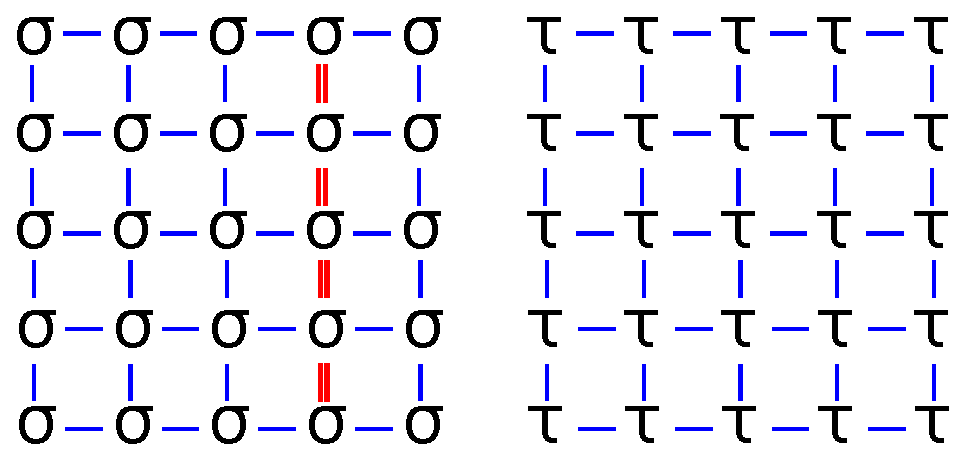
\includegraphics[scale=0.65]{graf/line_defect_sigma_tau_5x5.eps}
\end{center}
\caption{Defecto asim\'etrico en forma de línea. Los símbolos $\sigma$ y $\tau$ representan los diferentes tipos de spines y los segmentos que los unen
las constantes de acoplamiento entre ellos. La constante de acoplamiento entre los spines $\sigma$ se modifica sobre una l\'inea, indicada en color y con
 segmentos dobles, mientras que la constante de acoplamiento entre los spines $\tau$ conserva su valor en toda la red.}
\label{fig:line_defect_sigma}
\end{figure}

En este trabajo estudiaremos el comportamiento crítico local sobre un defecto con forma de línea en el modelo AT.
Introducimos un defecto asimétrico \cite{AT_naon} en el sistema modificando solo la interacción entre los spines de tipo $\sigma$ sobre una línea
del plano que los contiene (fig. \ref{fig:line_defect_sigma}), el acoplamiento entre los spines que yacen sobre el defecto y sus
 vecinos en la dirección perpendicular a la línea no se modifica, y dado que se trata del modelo AT 
 isotrópico, su valor $J$ es el mismo que para la interacción entre los spines $\tau$.
Llamando $J_{l}$ a la intensidad del defecto y considerando su contribución
 al Hamiltoniano del modelo AT (ec. \ref{eq:ham_AT}) en el caso isotrópico se obtiene:
\\
\begin{equation}
	\label{eq:line_pot}
	H_{AT}=-J\sum_{<ij,km>}(\sigma_{ij}\sigma_{km}+\tau_{ij}\tau_{km})-J_{4}\sum_{<ij,km>}\sigma_{ij}\sigma_{km}\tau_{ij}\tau_{km}-J_{l}\sum_{<ij,km>}\delta_{il}\sigma_{ij}\delta_{kl}\sigma_{km}
\end{equation}
donde las deltas en el último término hacen que la suma sea solo sobre los spines que se encuentran sobre la línea de defectos (sitios de la red con el primer índice igual a $l$).
De esta forma para $J_{l}=0$ se recupera el modelo AT sin defectos. La interacción entre los spines $\sigma$ que yacen sobre el defecto está dada por los términos primero y cuarto
 de este Hamiltoniano y por lo tanto el acoplamiento efectivo entre estos resulta $J+J_{l}$. Si bien el acoplamiento entre los spines $\tau$ no se modifica, el defecto tendrá influencia
 sobre su comportamiento debido a la conexión entre los spines $\sigma$ y los $\tau$ gobernada por la constante $J_{4}$.\\

Si se considera $K_{4}=0$ se obtienen dos modelos de Ising sin acoplamiento entre sí, uno con un defecto en forma de línea y otro sin defectos. El comportamiento
 del exponente crítico de la magnetización sobre la línea de defectos es diferente en cada uno de ellos. En el modelo con spines $\tau$ conserva su valor
 $\beta=\frac{1}{8}$ (el correspondiente al modelo de Ising), mientras que para los $\sigma$ se espera una dependecia del exponente con la intensidad del defecto $K_{l}=J_{l}/kT$:

\begin{equation}
	\label{eq:exp_crit_e0}
	x_{m}^{\sigma} = \frac{2}{\pi^{2}}arctan^{2}(e^{-2K_{l}}) , \; \; \; \; x_{m}^{\tau}=1/8, \; \; \; \; K_{4}=0.
\end{equation}
Esta relación fue hallada por Bariev \cite{AT_bariev_line} a partir de la solución exacta del modelo de Ising bidimensional con un defecto en forma de línea.\\

En el caso $K_{4}\neq 0$, la influencia del defecto sobre el comportamiento de los spines $\tau$ es gobernada por $K_{4}$. El comportamiento del
 exponente crítico de la magnetización asociado a ambos tipos de spines es algo complejo en este caso ya que la interacción efectiva entre los spines en la
 región en que el defecto se encuentra localizado depende de la competencia entre los acoplamientos $K$, $K_{4}$ y $K_{l}$. A continuación nos proponemos estudiar este
 comportamiento.\\

%El modelo de Ising bidimensional con un defecto en forma de línea fue estudiado por Bariev \cite{AT_bariev_line}, quien dedujo que el comportamiento de la magnetización
% local en función de la intensidad del defecto y la distancia a la línea, corresponde a leyes de potencia. Dado que para este modelo $d=2$, $d^{*}=1$ y $\nu=1$, el defecto
% resulta marginal y se espera que los exponentes críticos dependan de la intensidad del defecto.\\
%Bariev obtuvo esta dependencia para el exponente crítico de la magnetización sobre el defecto:
%\\
%\begin{equation}
%	\label{eq:exp_crit_bariev}
%	\beta_{l} = \frac{2}{\pi^{2}}arctan^{2}(e^{-2(K-K')}),
%\end{equation}
%\\

%donde $K$ es el acoplamiento entre spines del modelo de Ising y $K'$ el acoplamiento modificado, presente solo sobre el defecto.\\
